\documentclass[accentcolor=tud1b,colorbacktitle,landscape,german,presentation]{tudbeamer}

%Includes
\usepackage{float}
\usepackage{listings}
\usepackage{color}
\usepackage{graphicx}
\usepackage{epstopdf}
\usepackage{wrapfig}
\usepackage{pgfplots}
%Deutsche Silbentrennung
\usepackage[ngerman]{babel}
%Deutsche Umlaute
\usepackage[utf8]{inputenc}
\usepackage{adjustbox}
\usepackage{hyperref, tikz}
\usepackage{pdfpcnotes}

\setbeamerfont{note page}{size=\large}

\usetikzlibrary{shapes.misc, positioning, scopes}

\DeclareGraphicsExtensions{.pdf,.png,.jpg,.svg}
\graphicspath{ {./img/} }

\title[]{Entwicklung eines zentralen \\Steuerungsprogramms für einen \\Forschungsflugsimulator}
\subtitle{{\scriptsize Vortragender: Heiko Carrasco, Tim Weißmantel
	\\Team: Frederik Bark, Heiko Carrasco, Jonas Meurer, Tim Weißmantel und Leonardo Zaninelli}}
\institute{BP WS 2017/18 | Entwicklung eines zentralen Steuerungsprogramms für einen Forschungsflugsimulator}
\date{\today}

\newcommand{\ftitle}{
	\frametitle{\insertsectionhead \\ {\small \insertsubsectionhead}}
}

\pgfplotstableread[row sep=\\,col sep=&]{
	Iteration & Implementierung & Sonstiges & Storypoints\\
	0         &  6   & 29  & 0   \\
    1         &  51  & 26  & 40  \\
    2         &  64  & 17  & 17  \\
    3         &  88  & 29  & 60  \\
    4         &  104 & 16  & 33   \\
    5         &  0   & 0   & 0   \\
}\mydata

\begin{document}
%Deckblatt
\begin{titleframe}
	\begin{figure}
		\vspace{-18pt}
		\centering
		\includegraphics[scale=0.21]{simulator_3_intro}
	\end{figure}
	\pnote{Willkommen}
	\pnote{Gruppe 19}
\end{titleframe}


\section{Der Simulator}
\subsection{Aktuelle Situation}
\begin{frame}
	\ftitle
	\begin{figure}
		\centering
		\vspace{-.5cm}
		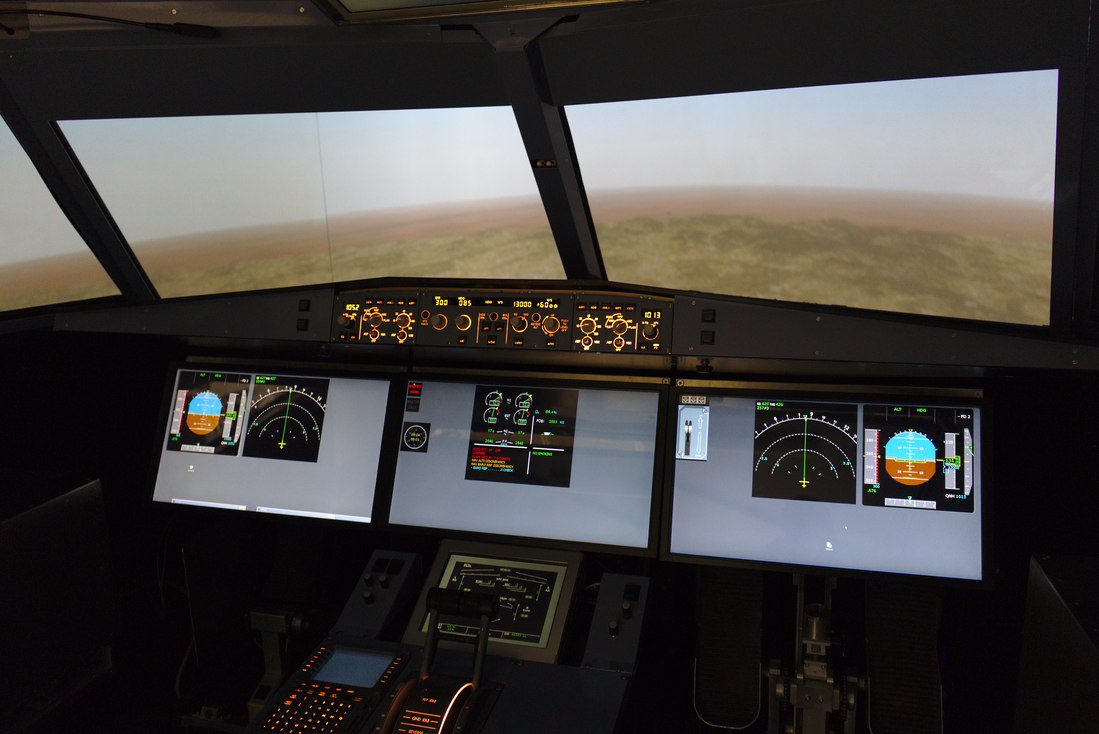
\includegraphics[]{sim-small}
	\end{figure}

	\pnote{Auftraggeber Institut für Flugsysteme und Regelungstechnik}
	\pnote{an der Lichtwiese}
	\pnote{wird zum Forschen im Bereich Führungsysteme (Flugverkehr) verwendet}
\end{frame}


\subsection{Aufbau des Systems}
\begin{frame}
	\ftitle
	\centering
	\begin{tikzpicture}[remember picture,overlay]
	\node[inner sep=0] at (current page.center)
	{		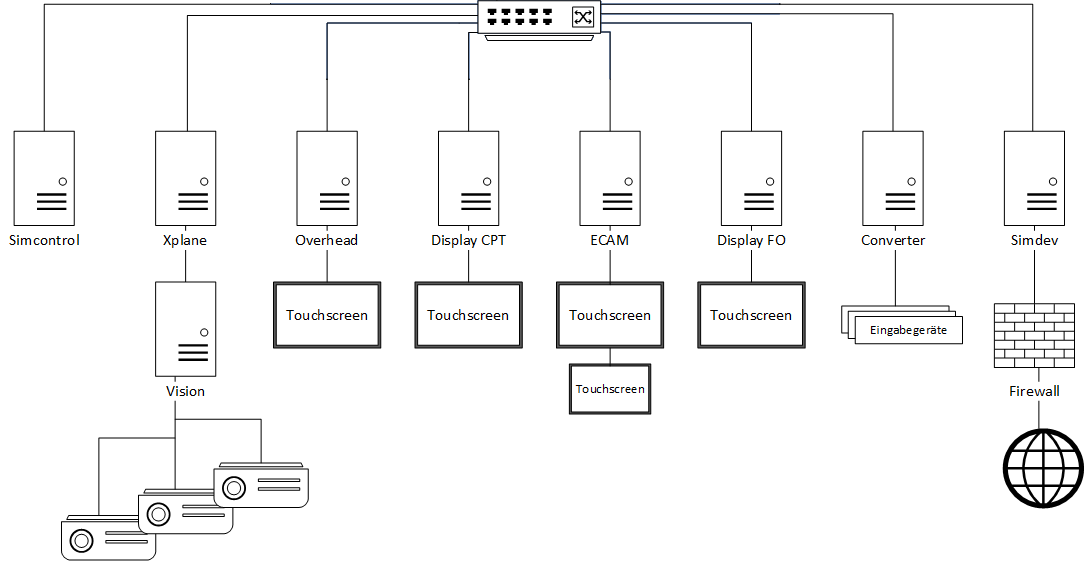
\includegraphics[scale=0.23]{aufbau_gesamt}};
	 \node (round) [line width=0.8pt,color=red, draw, rounded rectangle, yshift=-0.9cm, minimum height=1.3cm, minimum width=10cm] {};
		\node [color=red, below right= of round, yshift=0.9cm, xshift=-0.7cm] {Rechner};
	\end{tikzpicture}

\end{frame}

\subsection{Bisheriger Zustand}
\begin{frame}
	\ftitle
	\begin{overlayarea}{\textwidth}{.5\hsize}
	\begin{minipage}[t]{.7\textwidth}
	\begin{itemize}
		\item Jeder Rechner muss per Hand gestartet werden\pause
		\item Programme müssen einzeln gestartet werden\pause
			\begin{itemize}
				\item Nicht immer wird alles benötigt/darf gestartet werden\pause
				\item Viel Wechsel zwischen den Rechnern nötig
			\end{itemize}
	\end{itemize}
	\end{minipage}
	\begin{minipage}[t]{.2\textwidth}
		\onslide<1->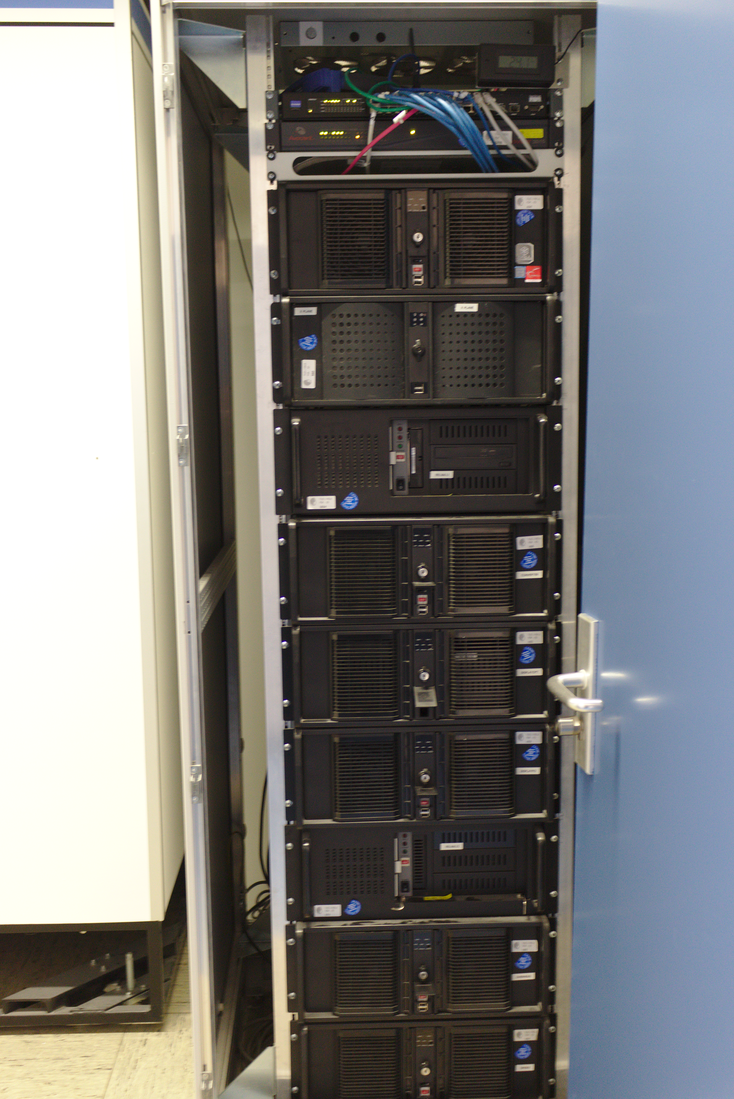
\includegraphics[scale=0.55]{server-small}
	\end{minipage}

	\end{overlayarea}
\end{frame}

\section{Software}
\subsection{Gewünschte Features}
\begin{frame}
	\ftitle
		Zentrale Oberfläche für...\\
			\begin{itemize}
				\item ...Steuern von Rechnern und Programmen\pause
				\item ...Statusübersicht\pause
				\item ...Programmierung von Startplänen\pause
			\begin{itemize}
				\item Szenarien (Flugplatz, Flugzeug, \dots) wählbar machen\pause
				\item Plugins laden oder deaktivieren
			\end{itemize}
			\end{itemize}
\end{frame}

\subsection{Lösung}
\begin{frame}
	\ftitle
	\centering
	\begin{tikzpicture}[node distance=2cm,v/.style={draw=blue, minimum size=7mm}, a/.style={circle,draw=blue!40,fill=blue!5,very thick, minimum size=5mm}, s/.style={circle, draw=green, fill=green!60, very thick, text=white, minimum size=7mm}, n/.style={midway, font=\footnotesize}]
		\visible<1->{\node[v] (Webinterface) {Webinterface};}
		\visible<2->{\node[v, draw=red, below = of Webinterface] (master) {Master};}
		\visible<3->{\node[v, draw=green, below left = of master] (client2) {Client 1};}
		\visible<3->{\node[v, draw=green, below right = of master] (client3) {Client 2};}

		\visible<4->{\draw[->, red] (Webinterface) to[bend right] node[n, left] {Kommandos} (master) ;}
		\visible<5->{\draw[->, red] (master.west) to[bend right] node[n, above left=8pt, yshift=-9pt, red] {Kommandos} (client2.north);}
		\visible<5->{\draw[->, red] (master.east) to[bend left] node[n, above right=8pt, yshift=-9pt, red] {Kommandos} (client3.north);}
		\visible<7->{\draw[->, blue] (master) to[bend right] node[n, right, blue] {Status} (Webinterface);}
		\visible<6->{\draw[->, blue] (client2.east) to[bend right] node[n, above left=4pt, yshift=-5pt, blue] {Status} (master.south);}
		\visible<6->{\draw[->, blue] (client3.west) to[bend left] node[n, above right=4pt, yshift=-5pt, blue] {Status} (master.south);}
	\end{tikzpicture}
\end{frame}


\subsection{Fortschritt}
\begin{frame}
	\ftitle
	\vspace{-0.8cm}
	\begin{figure}
		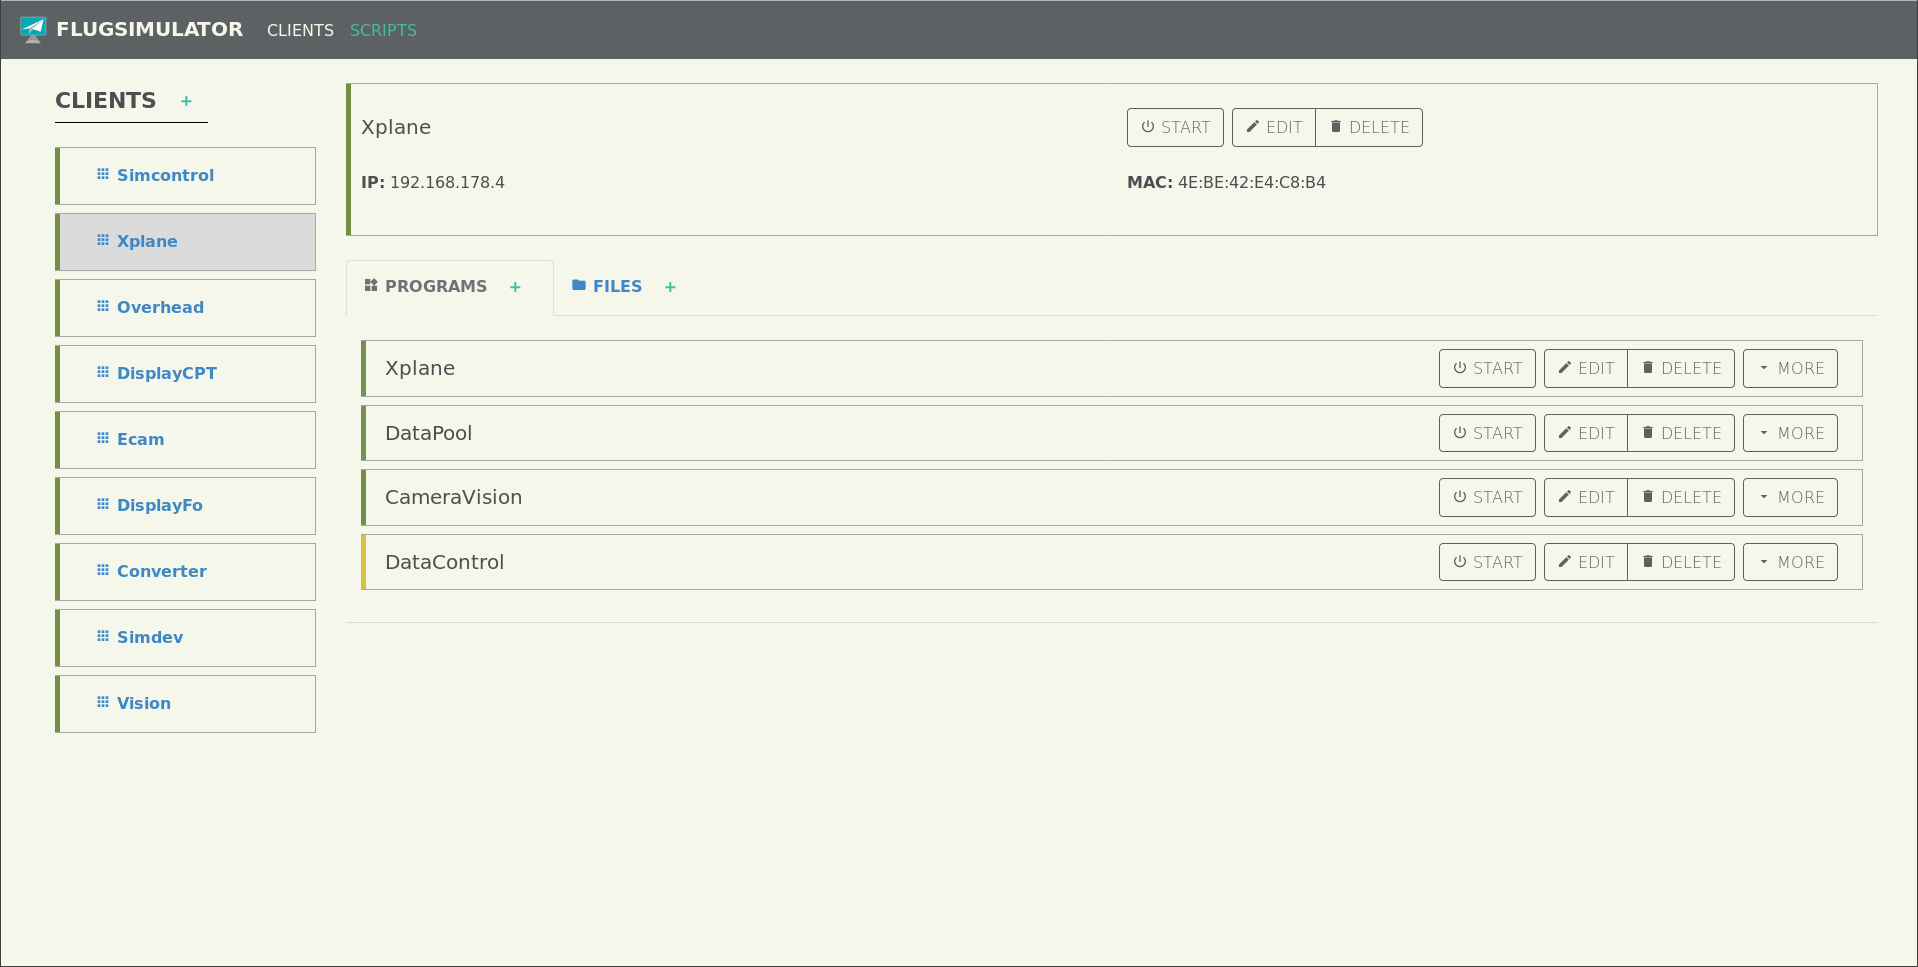
\includegraphics[scale=0.24]{interface}
	\end{figure}

	\pnote{hinzufügen von Clients im Webinterface}
	\pnote{hinzufügen von Programmen auf Clients im Webinterface}
	\pnote{wake on Lan}
	\pnote{grobe Implementierung von Master/Slave system}
\end{frame}

\section{Qualitätssicherung}
\subsection{Gesetzte Ziele}
\begin{frame}
	\ftitle
	\begin{itemize}
		\item Muss auf vielen unterschiedlichen Betriebssystem laufen
			\begin{itemize}
				\item <2->\textbf{Portabilität}
			\end{itemize}
		\item Einfache Bedienung für Mitarbeiter*innen
			\begin{itemize}
				\item <3->\textbf{Bedienbarkeit}
			\end{itemize}
		\item Muss weiterentwickelbar sein
			\begin{itemize}
				\item <4->\textbf{Korrektheit}
			\end{itemize}
	\end{itemize}

\end{frame}

\section{QS-Prozess}
\subsection{1. Automatisierte Tests}
\begin{frame}
	\ftitle
	\centering
	\vspace{-1.2cm}
	\begin{tikzpicture}
\node[inner sep=0pt] (marker) at (-4.45,2.3)
    {
\includegraphics[scale=0.06]{marker}};
\node[inner sep=0pt] (timeline) at (0,0)
    {\includegraphics[width=.8\textwidth]{qs-process}};
\end{tikzpicture}\pause
	\vspace{-4.5cm}
	\begin{itemize}
		\item QS-Ziele: \textbf{Portabilität, Korrekheit}\pause
	\end{itemize}
	\vspace{0.2cm}
	
\includegraphics[scale=0.2]{travisci}
	\hspace{0.1cm}
	
\includegraphics[scale=0.2]{appveyor}
	
\includegraphics[scale=0.18]{jenkins}
\end{frame}

\subsection{2. Coverage und Stilüberprüfung}
\begin{frame}
	\ftitle
	\centering
	\vspace{-1.2cm}
	\begin{tikzpicture}
\node[inner sep=0pt] (marker) at (-2.5,2.3)
    {
\includegraphics[scale=0.06]{marker}};
\node[inner sep=0pt] (timeline) at (0,0)
    {\includegraphics[width=.8\textwidth]{qs-process}};
\end{tikzpicture}\pause
	\vspace{-4.5cm}
	\begin{itemize}
		\item QS-Ziel: \textbf{Korrektheit}\pause
	\end{itemize}
	\vspace{0.2cm}
	
\includegraphics[scale=0.2]{coveralls}
	\hspace{0.1cm}
	
\includegraphics[scale=0.14]{codacy}
\end{frame}


\begin{frame}
	\ftitle
	\vspace{-0.5cm}
	\begin{figure}
		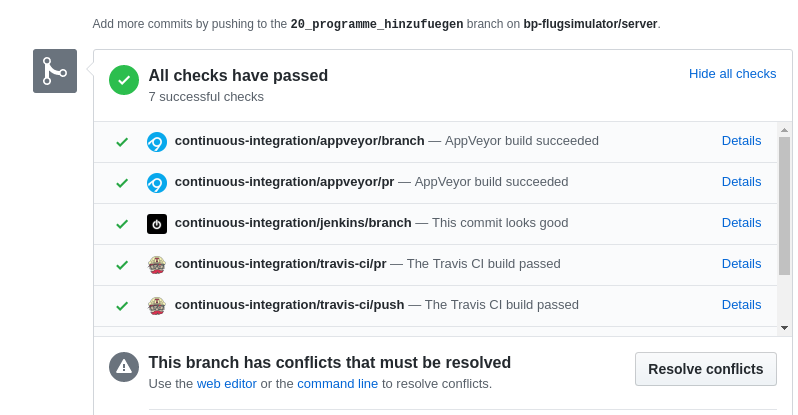
\includegraphics[scale=0.4]{github_integration}
	\end{figure}

	\pnote{für jede Userstory wird ein Pullrequests auf Github gemacht}
	\pnote{dient auch als Forum für Implementierungen}
\end{frame}

\subsection{3. Review durch anderen Entwickler}
\begin{frame}
	\ftitle
	\centering
	\vspace{-1.2cm}
	\begin{tikzpicture}
\node[inner sep=0pt] (marker) at (-0.55,2.3)
    {
\includegraphics[scale=0.06]{marker}};
\node[inner sep=0pt] (timeline) at (0,0)
    {\includegraphics[width=.8\textwidth]{qs-process}};
\end{tikzpicture}
	\vspace{-4.5cm}
	\begin{itemize}
		\item Review wird von einem anderen Entwickler durchgeführt\pause
		\item Checkliste mit Punkten wie z.B. Dokumentation
	\end{itemize}
\end{frame}

\begin{frame}
	\ftitle
	\begin{figure}
		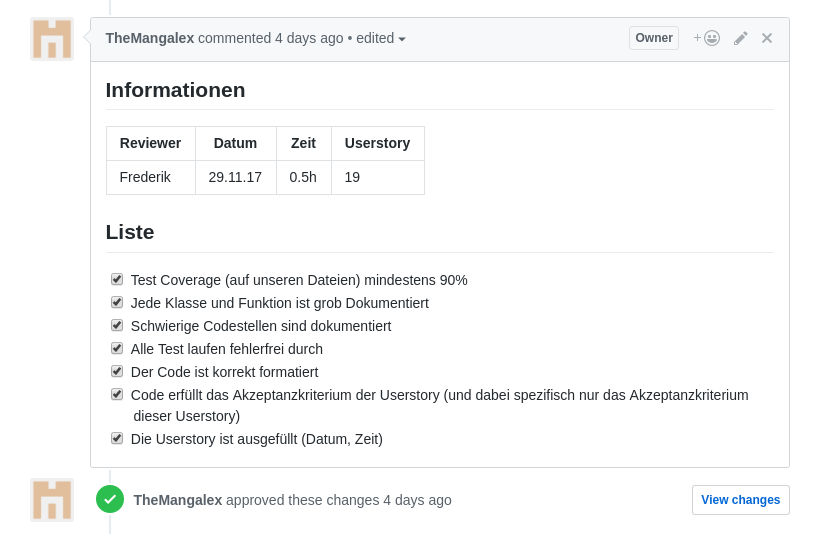
\includegraphics[scale=0.29]{github_list}
	\end{figure}
	\pnote{falls eine Punkt nicht erfüllt wird, muss der Entwickler der Userstory
		das Problem beheben}
\end{frame}

\subsection{4. Nutzerstudie am Fachgebiet}
\begin{frame}
	\ftitle
	\centering
	\vspace{-1.2cm}
	\begin{tikzpicture}
\node[inner sep=0pt] (marker) at (1.42,2.3)
    {
\includegraphics[scale=0.06]{marker}};
\node[inner sep=0pt] (timeline) at (0,0)
    {\includegraphics[width=.8\textwidth]{qs-process}};
\end{tikzpicture}
	\vspace{-4.5cm}
	\begin{itemize}
		\item QS-Ziel: \textbf{Bedienbarkeit}\pause
		\item Nutzerstudie zum Test der Bedienbarkeit\pause
		\item Durchführung Anfang 2018
	\end{itemize}
\end{frame}


\subsection{5. Abnahme durch die Auftraggeber}
\begin{frame}
	\ftitle
	\centering
	\vspace{-1.2cm}
	\begin{tikzpicture}
\node[inner sep=0pt] (marker) at (3.39,2.3)
    {
\includegraphics[scale=0.06]{marker}};
\node[inner sep=0pt] (timeline) at (0,0)
    {\includegraphics[width=.8\textwidth]{qs-process}};
\end{tikzpicture}
	\vspace{-4.5cm}
	\begin{itemize}
		\item Auftraggeber erhalten Zusammenfassung\pause
		\item Anmerkungen für die nächste Iteration
	\end{itemize}
\end{frame}

\section{Zeiterfassung}

\begin{frame}
	\ftitle
	\begin{figure}
			\begin{tikzpicture}
				\begin{axis}
					[
            		ybar,
            		bar width=.5cm,
            		width=\textwidth,
					height=.5\textwidth,
					legend style={at={(0.5,1)}, anchor=north,legend columns=-1},
            		symbolic x coords={0,1,2,3,4,5},
            		xtick=data,
            		nodes near coords,
            		nodes near coords align={vertical},
            		ylabel={Stunden},
					xlabel={Iteration},
					ymax=150,
        		]
        		\addplot table[x=Iteration,y=Implementierung]{\mydata};
        		\addplot table[x=Iteration,y=Sonstiges]{\mydata};
				\addplot table[x=Iteration,y=Storypoints]{\mydata};
				\legend{Implementierung, Sonstiges, Storypoints}
    		\end{axis}
		\end{tikzpicture}
	\end{figure}

	\pnote{Willkommensnachricht wurde stark überschätzt}
	\pnote{für Slaves registrieren gab es 3 verschiedenen Ansätze die viel Diskutiert wurden}
	\pnote{in Slaves löschen und Slaves registrieren wurde viel Vorarbeit für Slaves bearbeiten  gemacht}
\end{frame}

\section{Fragen}
\begin{frame}
	\ftitle
	\vspace{-10pt}
	\centering
	\begin{figure}
		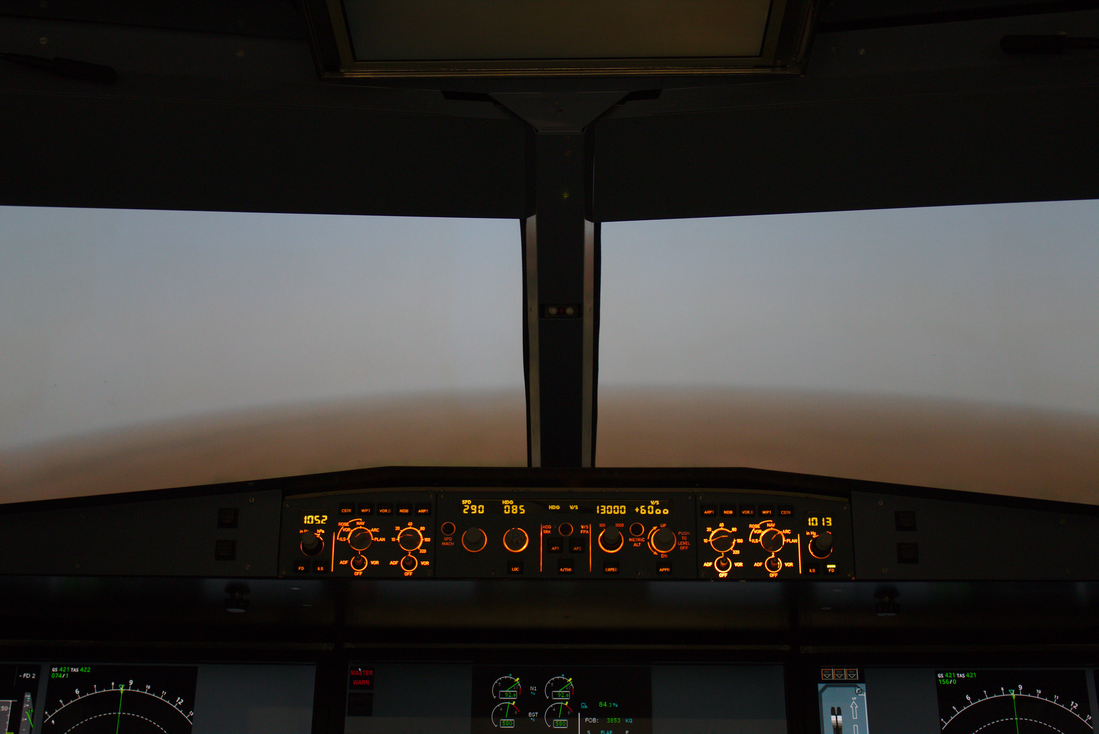
\includegraphics[scale=0.8]{console-small}
	\end{figure}
\end{frame}

\section{Table of Contents}
\begin{frame}[allowframebreaks]
	\ftitle
	\tableofcontents
\end{frame}

\end{document}
